\documentclass[10pt, twocolumn]{scrreprt}

% Gib die Versuschsnummer an, um den entsprechenden Versuchsprotokoll zu laden
\newcommand{\versuchsnummer}{11}
\usepackage{Versuchs_Informationen}
\usepackage{style}


\begin{document}
\begin{titlepage}
\vspace*{2cm} 
  
  \centering
    
  % Versuchs-Titel
  {\LARGE\bfseries Protokoll zum Versuch \\[0.2cm]
  \textit{\versuchsname{\versuchsnummer}} \\[0.5cm] % Vielleicht wieder Anführungszeichen hinzufügen, leider Problem, da ein Leerzeichen falsch hinzugefügt wird.
  {\large (Versuch {\versuchsnummer})}
  \vspace{1cm}}

  % Tabelle mit Metadaten
  {\large
  \begin{tabular}{@{}rl@{}}
    Autor:                  & Finn Zeumer (hz334)\\
    Versuchspatnerin        & Annika Künstle\\[0.5em]
    Versuchsbegleiter:      & {\begleiter{\versuchsnummer}}\\[0.5em]
    Datum der Ausführung:   & {\durchfuehrungsdatum{\versuchsnummer}}\\
    \small{Abgabedatum:}    & \small{\abgabedatum{\versuchsnummer}}\\
  \end{tabular}
  }
  \vfill


  \begin{tikzpicture}[remember picture,overlay]
    \node[opacity=1,inner sep=0] at (current page.center)
      {
\includegraphics[width=\paperwidth,height=\paperheight]{hd-img/Titelhintergund_7_Page 2.png}};
  \end{tikzpicture}
  
\end{titlepage} 
% \onecolumn
\section{Fehlerrechnung}
Für die statistische Auswertung von $n$ Messwerten $x_i$ werden folgende Größen definiert \cite{errorSkript25}:
\begin{align}
    \bar{x} &= \frac{1}{n} \sum_{i=1}^{n} x_i \vphantom{\sqrt{\sum_i^n}^2} && \text{\textcolor{gray}{Arithmetisches Mittel}} \label{eq:arithmetisches_mittel} \\
    \sigma^2 &= \frac{1}{n-1} \sum_{i=1}^{n} (x_i - \bar{x})^2 \vphantom{\sqrt{\sum_i^n}^2} && \text{\textcolor{gray}{Variation}} \label{eq:variation} \\
    \sigma &= \sqrt{\frac{1}{n-1} \sum_{i=1}^{n} (x_i - \bar{x})^2} \vphantom{\sqrt{\sum_i^n}^2} && \text{\textcolor{gray}{Standardabweichung}} \label{eq:standardabweichung} \\
    \Delta \bar{x} &= \frac{\sigma}{\sqrt{n}} = \sqrt{\frac{1}{n(n-1)} \sum_{i=1}^n(\bar x - x_i)^2} \vphantom{\sqrt{\sum_i^n}^2} && \text{\textcolor{gray}{Fehler des Mittelwerts}} \label{eq:fehler_mittelwert} \\
    \Delta f &= \sqrt{\left(\frac{\partial f}{\partial x} \Delta x\right)^2 + \left(\frac{\partial f}{\partial y} \Delta y\right)^2} \vphantom{\sqrt{\sum_i^n}^2} && \text{\textcolor{gray}{Gauß’sches Fehlerfortpflanzungsgesetz für $f(x,y)$}} \label{eq:gauss_fehlfortpflanzung} \\
    \Delta f &= \sqrt{(\Delta x)^2 + (\Delta y)^2} \vphantom{\sqrt{\sum_i^n}^2} && \text{\textcolor{gray}{Fehler für $f = x + y$}} \label{eq:fehler_summe} \\
    \Delta f &= |a| \Delta x \vphantom{\sqrt{\sum_i^n}^2} && \text{\textcolor{gray}{Fehler für $f = ax$}} \label{eq:fehler_proportional} \\
    \frac{\Delta f}{|f|} &= \sqrt{\left(\frac{\Delta x}{x}\right)^2 + \left(\frac{\Delta y}{y}\right)^2} \vphantom{\sqrt{\sum_i^n}^2} && \text{\textcolor{gray}{relativer Fehler für $f = xy$ oder $f = x/y$}} \label{eq:relativer_fehler} \\
    \sigma &= \frac{|a_{lit} - a_{gem}|}{\sqrt{\Delta a_{lit}^2 + \Delta a_{gem}^2}} \vphantom{\sqrt{\sum_i^n}^2} && \text{\textcolor{gray}{Berechnung der signifikanten Abweichung}} \label{eq:signifikante_abweichung}
\end{align}

\twocolumn

\renewcommand{\contentsname}{Inhaltsverzeichnis}
\tableofcontents

% Lade die Versuchsnummer-spezifischen Informationen
\addcontentsline{toc}{chapter}{Measurement Data} 
\label{protocol}

% \thispagestyle{empty}

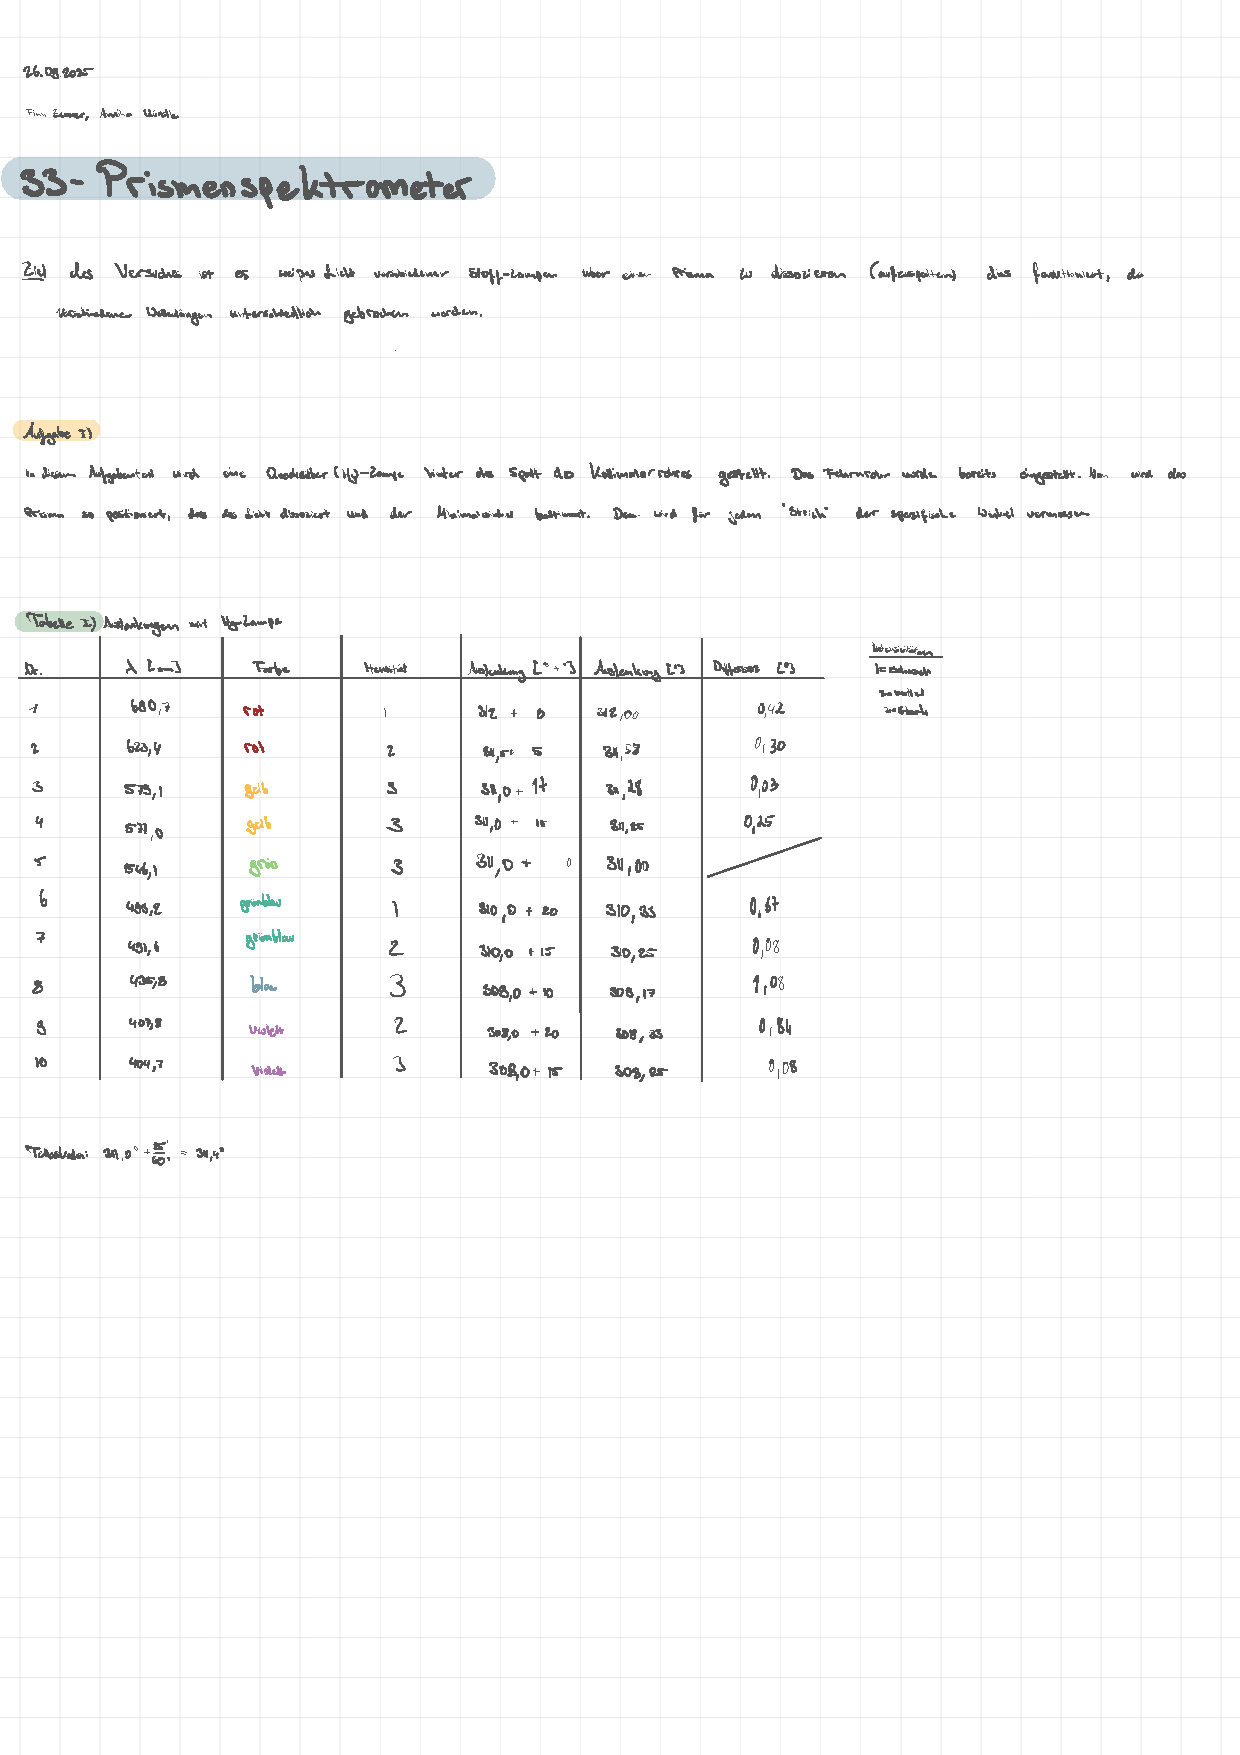
\includepdf[
  pages=1-3,               
  pagecommand={\thispagestyle{empty}} 
]{Protokolle/\versuchsnummer/Chapter/Messprotokoll.pdf}

\addcontentsline{lot}{table}{\protect\numberline{\thechapter.1} Materialeigenschaften}
\addcontentsline{lot}{table}{\protect\numberline{\thechapter.2} Messreihe des Wasserkalorimeters zur Bestimmung des Wasserwertes}
\addcontentsline{lot}{table}{\protect\numberline{\thechapter.3} Messreihe im Wasserkalorimeters Aluminium}
\addcontentsline{lot}{table}{\protect\numberline{\thechapter.4} Messreihe im Wasserkalorimeters Blei}
\addcontentsline{lot}{table}{\protect\numberline{\thechapter.5} Messreihe im Wasserkalorimeters Graphit}
\addcontentsline{lot}{table}{\protect\numberline{\thechapter.5} Messreihe der Körper im Flüssigstickstoff}

\chapter{Einleitung}

\section{Aufgabe/Motivation}
Ziel des Versuchs ist die Bestimmung des Richtmoments $D$ eines Drehpendels sowie die Untersuchung des Trägheitsmoments $J$ eines unregelmäßig geformten Körpers für verschiedene Lagen der Drehachse. Dazu wird einerseits das Richtmoment über die Auslenkung des Pendels durch ein angreifendes Drehmoment bestimmt, andererseits über die Periodendauer einer Schwingung mit aufgesetzten Körpern bekannter Geometrie. Mit Hilfe des Steiner’schen Satzes lässt sich schließlich das Trägheitsmoment für verschiedene Achsen berechnen und mit den experimentell gewonnenen Werten vergleichen.

\section{Physikalische Grundlagen}
\subsection*{Analogie zwischen Translations- und Rotationsbewegung}
Die Bewegungsgleichungen für Translationen und Rotationen sind formal analog, wenn die entsprechenden Größen ausgetauscht werden. Dabei gilt:

\begin{table}[h!]
\renewcommand{\arraystretch}{1.75} % Zeilenhlöhe
\centering
\begin{tabular}{l|l}
    \textbf{Translation} & \textbf{Rotation} \\
    \hline
    Ort $x$ & Winkel $\varphi$ \\
    Geschwindigkeit $v = \tfrac{dx}{dt}$ & Winkelges. $\omega = \tfrac{d\varphi}{dt}$ \\
    Beschleunigung $a = \tfrac{d^2x}{dt^2}$ & Winkelbes. $\alpha = \tfrac{d^2\varphi}{dt^2}$ \\
    Masse $m$ & Trägheitsmoment $J$ \\
    Kraft $F$ & Drehmoment $M$ \\
    Impuls $p = mv$ & Drehimpuls $L = J\omega$ \\
    Trans.En. $E_{kin} = \tfrac{1}{2}mv^2$ & Rot.En. $E_{rot} = \tfrac{1}{2}J\omega^2$ \\
\end{tabular}
\caption{Vergleich der Größen in der Translation und Rotation}
\label{tab:translation-rotation}
\end{table}

\vspace{0.25cm}

Auch Federpendel und Drehpendel stehen in direkter Analogie:

\begin{equation}
    F = -kx \quad \Leftrightarrow \quad M = -D\varphi
\end{equation}

\begin{equation}
T = 2\pi\sqrt{\frac{m}{k}} \quad \Leftrightarrow \quad T = 2\pi\sqrt{\frac{J}{D}}
\end{equation}

Das Richtmoment $D$ spielt dabei die Rolle der Federkonstante $k$.

\subsection*{Trägheitsmoment}
Das Trägheitsmoment $J$ eines Körpers bezüglich einer gegebenen Drehachse ergibt sich aus dem Volumenintegral:

\begin{equation}
    J = \int_V \rho(\vec{r}) r^2 \, dV,
\end{equation}

wobei $\rho(\vec{r})$ die Massendichte und $r$ der Abstand des Volumenelements zur Achse ist.  
Für einfache Körper ergeben sich bekannte Spezialfälle, etwa für eine homogene Scheibe mit Masse $m$ und Radius $r_s$:

\begin{equation}
    J_S = \tfrac{1}{2} m r_s^2
\end{equation}

Hierbei ist $J_S$ das Trägheitsmoment der Scheibe, $m$ ihre Masse und $r_s$ ihr Radius.

\subsection*{Steiner’scher Satz}
Für eine Achse, die parallel zur Symmetrieachse im Abstand $d$ verläuft, gilt:

\begin{equation}
    J = J_S + md^2
\end{equation}

mit $J_S$ als Trägheitsmoment bezüglich der Symmetrieachse, $m$ als Masse des Körpers und $d$ als Abstand der Achsen.

\subsection*{Bestimmung des Richtmoments}
Das Richtmoment $D$ des Drehpendels kann auf zwei Weisen bestimmt werden:

\begin{enumerate}
    \item Über das Kraftgesetz:
    \begin{equation}
        M = r \cdot F = -D\varphi,
    \end{equation}
    wobei $M$ das Drehmoment, $r$ der Radius der Aluminiumscheibe, $F = mg$ die Gewichtskraft eines tangential angreifenden Massestücks und $\varphi$ der Auslenkwinkel ist.
    
    \item Über die Schwingungsdauer $T$ mit bekannter Massescheibe:
    \begin{equation}
        D = \frac{4\pi^2 J_S}{T_2^2 - T_1^2} = \frac{2\pi^2 m r_s^2}{T_2^2 - T_1^2},
    \end{equation}
    wobei $T_1$ die Periodendauer des Tisches allein, $T_2$ die Periodendauer mit aufgesetzter Scheibe, $J_S$ das Trägheitsmoment der Scheibe, $m$ ihre Masse und $r_s$ ihr Radius ist.
\end{enumerate}

\section{Versuchsanordnung}
    Der Versuch wird mit einem Drehpendel mit senkrechter Achse durchgeführt. Zum Aufbau gehören eine Drehgabel mit Drehtisch, eine Aluminiumscheibe mit Winkelteilung und Schnurnut, eine runde sowie eine unregelmäßig geformte Messingscheibe, ein Gewichtsteller mit Zugschnur, sechs Auflegegewichte zu je 40 g, eine Waage, eine Handstoppuhr, ein Messschieber sowie eine Balancierschneide. Mit diesem Aufbau lassen sich die notwendigen Messungen zur Bestimmung des Richtmoments und der Trägheitsmomente der untersuchten Körper durchführen.

\chapter{Durchführung}

\section{Versuchsaufbau}

\subsection*{Aufgabe 1: Eichung der Thermometer bei 0\,°C}
Für die Eichung wird ein Pt100-Thermometer mit Adapterbox verwendet. Die vier Anschlussleitungen können über 4\,mm-Buchsen abgegriffen werden. Eine Stromquelle liefert den Messstrom von 1\,mA. Ein Voltmeter dient zur Spannungsmessung und kann wahlweise an die Buchsen der Stromquelle (Zweileiterschaltung) oder direkt an die Adapterbox (Vierleiterschaltung) angeschlossen werden.  
Zur Erzeugung der Referenztemperatur von 0\,°C wird ein Becherglas mit zerkleinertem Eis und Wasser befüllt. Der Glasballon mit dem Messsensor wird vollständig in das Gemisch eingetaucht. Zusätzlich stehen ein Pyrometer zur Messung der Oberflächentemperatur sowie ein Flüssigkeitsthermometer zur Verfügung.

\subsection*{Aufgabe 2: Temperaturmessung bis 100\,°C}
Das Wasserbad wird mit einer Heizplatte erhitzt. Zur Temperaturhomogenisierung wird ein Rührmechanismus verwendet. Als Messgeräte dienen das Pt100-Thermometer, das Gasthermometer und ein Pyrometer. Der Umgebungsdruck wird mit einem Barometer bestimmt.

\subsection*{Aufgabe 3: Temperaturmessung bei tiefen Temperaturen}
Ein Dewargefäß wird wahlweise mit einer Trockeneis-Alkohol-Mischung oder mit flüssigem Stickstoff befüllt. Der Glasballon mit Messsensor wird in das jeweilige Kühlmedium eingebracht. Für die Messung stehen das Pt100-Thermometer sowie das Gasthermometer zur Verfügung.

\subsection*{Aufgabe 4: Temperaturmessung mit dem PtRh-Thermoelement}
Zur Untersuchung hoher Temperaturen wird ein Gasbrenner mit regelbarer Luftzufuhr genutzt. Das PtRh-Thermoelement (Typ S oder Typ B) wird in verschiedene Bereiche der Flamme eingeführt. Die Temperaturbestimmung erfolgt über die gemessene Thermospannung unter Zuhilfenahme der passenden Eichtabelle.

\section{Messverfahren}


Nach dem Aufbau der Zwei- und Vierleiterschaltung werden beide Varianten ausprobiert. Bei stabilisierter Temperatur im Wasser-Eis-Gemisch wird die Spannung des Pt100, der Druck des Gasthermometers sowie die Pyrometertemperatur aufgezeichnet. Das Flüssigkeitsthermometer wird als zusätzliche Kontrolle herangezogen. Maßgeblich ist das Minimum der Pt100-Spannung als Eichpunkt.


Das Wasser wird stufenweise erhitzt. Beginnend bei etwa 10\,°C werden in Schritten von ca. 10\,°C die Pt100-Spannung, der Gasthermometerdruck und die Pyrometertemperatur aufgenommen. Als letzter Messpunkt dient die Temperatur des siedenden Wassers. Der Luftdruck wird parallel am Barometer erfasst. Das Pyrometer wird schräg auf die Wasseroberfläche gerichtet, um Verfälschungen durch Wasserdampf zu vermeiden.


Zunächst wird die Trockeneis-Alkohol-Mischung genutzt. Nach ausreichender Abkühlung und Temperaturstabilisierung werden Pt100-Spannung und Druck protokolliert. Anschließend wird der Versuch mit flüssigem Stickstoff wiederholt. Der Glasballon wird vollständig eingetaucht und die Messwerte nach Abklingen der starken Verdampfung notiert. Das Pyrometer wird nicht eingesetzt, da es bei diesen Temperaturen unbrauchbar ist.

\subsection*{Aufgabe 4: Temperaturmessung mit dem PtRh-Thermoelement}
Das Thermoelement wird in die Flamme des Gasbrenners eingeführt. Bei starker und schwacher Luftzufuhr werden jeweils mehrere Messpunkte in unterschiedlichen Flammenzonen untersucht. Für jeden Punkt wird die Thermospannung bestimmt. Die Flammenform wird zusätzlich skizziert und mit den Messwerten ergänzt. Die Umrechnung in Temperatur erfolgt anhand der für den verwendeten Thermoelementtyp gültigen Eichtabelle.

\onecolumn
\chapter{Auswertung}
% Liste der genutzer Formeln für die Fehlerrechnung
\section*{Fehlerrechnung}
Für die statistische Auswertung von $n$ Messwerten $x_i$ werden folgende Größen definiert \cite{errorSkript25}:
\begin{align}
    \bar{x} &= \frac{1}{n} \sum_{i=1}^{n} x_i \vphantom{\sqrt{\sum_i^n}^2} && \text{\textcolor{gray}{Arithmetisches Mittel}} \label{eq:arithmetisches_mittel} \\
    \sigma^2 &= \frac{1}{n-1} \sum_{i=1}^{n} (x_i - \bar{x})^2 \vphantom{\sqrt{\sum_i^n}^2} && \text{\textcolor{gray}{Variation}} \label{eq:variation} \\
    \sigma &= \sqrt{\frac{1}{n-1} \sum_{i=1}^{n} (x_i - \bar{x})^2} \vphantom{\sqrt{\sum_i^n}^2} && \text{\textcolor{gray}{Standardabweichung}} \label{eq:standardabweichung} \\
    \Delta \bar{x} &= \frac{\sigma}{\sqrt{n}} = \sqrt{\frac{1}{n(n-1)} \sum_{i=1}^n(\bar x - x_i)^2} \vphantom{\sqrt{\sum_i^n}^2} && \text{\textcolor{gray}{Fehler des Mittelwerts}} \label{eq:fehler_mittelwert} \\
    \Delta f &= \sqrt{\left(\frac{\partial f}{\partial x} \Delta x\right)^2 + \left(\frac{\partial f}{\partial y} \Delta y\right)^2} \vphantom{\sqrt{\sum_i^n}^2} && \text{\textcolor{gray}{Gauß’sches Fehlerfortpflanzungsgesetz für $f(x,y)$}} \label{eq:gauss_fehlfortpflanzung} \\
    \Delta f &= \sqrt{(\Delta x)^2 + (\Delta y)^2} \vphantom{\sqrt{\sum_i^n}^2} && \text{\textcolor{gray}{Fehler für $f = x + y$}} \label{eq:fehler_summe} \\
    \Delta f &= |a| \Delta x \vphantom{\sqrt{\sum_i^n}^2} && \text{\textcolor{gray}{Fehler für $f = ax$}} \label{eq:fehler_proportional} \\
    \frac{\Delta f}{|f|} &= \sqrt{\left(\frac{\Delta x}{x}\right)^2 + \left(\frac{\Delta y}{y}\right)^2} \vphantom{\sqrt{\sum_i^n}^2} && \text{\textcolor{gray}{relativer Fehler für $f = xy$ oder $f = x/y$}} \label{eq:relativer_fehler} \\
    \sigma &= \frac{|a_{lit} - a_{gem}|}{\sqrt{\Delta a_{lit}^2 + \Delta a_{gem}^2}} \vphantom{\sqrt{\sum_i^n}^2} && \text{\textcolor{gray}{Berechnung der signifikanten Abweichung}} \label{eq:signifikante_abweichung}
\end{align}

\twocolumn

\section{Fehlerbestimmung zweier Messmethoden}
Zunächst werden die beiden Methoden unabhänig voneinander ausgewertet und die Ergebnisse miteinander verglichen. Ziel ist es, die Methode mit der geringeren Unsicherheit zu identifizieren und diese für die weiteren Messungen zu verwenden.
\subsection*{Methode 1}
Wir schauen uns zunächst die erste Methode an, bei der die Periodendauer $T_{m}$ über die maximale Auslenkung des Pendels gemessen wird. Die Messwerte sind aus dem Protokoll \ref{Protokoll} entnommen. Die in Tabelle \ref{tab:max_Auslenkung} aufgelisteten Werte sind auf die Wesentlichen beschrängt.
Dabei ist $T_{m}$ die gemessene Periodendauer, $\Delta T_{m}T$ der absolute Fehler und $\Delta T_{m} (\%)$ der relative Fehler in Prozent.
\messwertetabelle
\vspace{2pt}
Der Mittelwert der Periodendauer beträgt:
\begin{equation}
    \bar{T}_{m} = \frac{1}{\anzahlmesswerte}\sum_{i=1}^{\anzahlmesswerte} T_{m,i} = \underline{\mittelwert\,\mathrm{s}}.
\end{equation}
Über diesen Mittelwert sind auch die Abweichungen der Einzelwerte $\Delta T$ berechnet.

Der mittlere Fehler des Mittelwerts berechnet sich zu:
\begin{align}
    \Delta \bar{T}_{m} &= \sqrt{\frac{1}{10(10-1)} \sum_{i=1}^{10} (\bar{x}-x_i)^2}  \\
    \Delta \bar{T}_{m} &= \underline{\statistischerfehler\,\mathrm{s}}
\end{align}

Wir kommen also zu dem Ergebnis:
\begin{equation}
    \underline{\underline{T_{m} = \bar{T}_{m} \pm \Delta \bar{T}_{m} = (1,587 \pm 0,014)\,\mathrm{s}.}}
\end{equation}

\subsection*{Methode 2}
Nun vergleichen wir das mit der zweiten Methode, bei der die Periodendauer $T_{n}$ über den Nulldurchgang des Pendels gemessen wird. Die Messwerte sind aus dem Protokoll \ref{Protokoll} entnommen. Die in Tabelle \ref{tab:null_Auslenkung} aufgelisteten Werte sind auf die Wesentlichen beschrängt.
\begin{table}[h!]
\centering

\begin{tabular}{c|c|c|c}
Messung & $T_{n} [s]$ & $\Delta T_{n} [s]$ & $\Delta T_{n} [\%]$ \\
\hline
1 & 1,687 & -0,002 & -0,12 \\
2 & 1,713 & 0,024 & 1,42 \\
3 & 1,697 & 0,008 & 0,47 \\
4 & 1,713 & 0,024 & 1,42 \\
5 & 1,713 & 0,024 & 1,42 \\
6 & 1,697 & 0,008 & 0,47 \\
7 & 1,643 & -0,046 & -2,72 \\
8 & 1,687 & -0,002 & -0,12 \\
9 & 1,673 & -0,016 & -0,95 \\
10 & 1,667 & -0,022 & -1,30 \\
\hline
$\bar{T}_{n}$ & 1,689 & & \\
\end{tabular}
\caption{Periodendauer berechnet durch die Messung bei Nullauslenkung des Pendels}
\label{tab:null_Auslenkung}
\end{table}

Der Mittelwert der Periodendauer beträgt:
\begin{equation}
    \bar{T}_{n} = \frac{1}{\anzahlmesswerte}\sum_{i=1}^{\anzahlmesswerte} T_{n,i} = \underline{1,689\,\mathrm{s}}.
\end{equation}
Über diesen Mittelwert sind wieder die Abweichungen der Einzelwerte $\Delta T_{n}$ berechnet.
Der mittlere Fehler des Mittelwerts berechnet sich zu:
\begin{align}
    \Delta \bar{T}_{n} & = \sqrt{\frac{1}{10(10-1)} \sum_{i=1}^{10} (\bar{x}-x_i)^2} \\
    \Delta \bar{T}_{n} & = \underline{0,096\,\mathrm{s}}.
\end{align}

Für die zweite Methode ergibt sich somit:
\begin{equation}
    \underline{\underline{T_{n} = \bar{T}_{n} \pm \Delta \bar{T}_{n} = (1,689 \pm 0,096)\,\mathrm{s}.}} 
\end{equation}

\subsection*{Vergleich der Methoden}
Nun können wir die beiden Methoden miteinander vergleichen. Die erste Methode liefert eine Periodendauer von $T_{m} = (1,587 \pm 0,014)\,\mathrm{s}$, während die zweite Methode eine Periodendauer von $T_{n} = (1,689 \pm 0,096)\,\mathrm{s}$ ergibt.
Über die Werte bestimmen wir nun die Standardabweichung \eqref{eq:standardabweichung} des Mittelwertes. Die kleinere Standardabweichung deutet auf die genauere Methode hin:
\begin{align}
    \sigma_{\bar{T}_m} &= \sqrt{\frac{1}{9} \sum_{i=1}^{10} (\bar{T_m}-T_{m,i})^2} = \underline{0,043\,\mathrm{s}} \\
    \sigma_{\bar{T}_n} &= \sqrt{\frac{1}{9} \sum_{i=1}^{10} (\bar{T_n}-T_{n,i})^2} = \underline{0,030\,\mathrm{s}}
\end{align}

Eindeutig zusehen ist, dass Methode 2, also die Messung über den \emph{Nulldurchgang} die kleinere Standardabweichung aufweist und somit die genauere Methode ist. Diese wird im Folgenden für die weiteren Messungen verwendet.

\section{Messen der Schwingungsdauer als Funktion der Masse}
Nun geht es zum nächsten Schritt: die Abhängigkeit der Schwingungsdauer $T$ von der angehängten Masse $m$ zu untersuchen. Die Messwerte sind aus dem Protokoll \ref{Protokoll} entnommen. Die in Tabelle \ref{tab:verschiedene_massen_messungen} aufgelisteten Werte sind auf die Wesentlichen beschrängt.
Das Ziel ist es eine Funktion in Abhängigkeit der Federkonstante $D$ zu bestimmen.

\begin{table}[h!]
    \centering
    \begin{tabular}{c | c | c | c}
    Masse [g] & $T$ [s] & $\Delta T$ [s] & $\Delta \bar{T}$ [s] \\
    \hline
    50  & 0,927 & 0,933 & 0,004 \\
        & 0,933 &       &       \\
        & 0,940 &       &       \\
    \hline
    100 & 1,213 & 1,218 & 0,004 \\
        & 1,213 &       &       \\
        & 1,227 &       &       \\
    \hline
    150 & 1,500 & 1,501 & 0,005 \\
        & 1,510 &       &       \\
        & 1,493 &       &       \\
    \hline
    200 & 1,673 & 1,680 & 0,014 \\
        & 1,707 &       &       \\
        & 1,660 &       &       \\
    \hline
    250 & 1,863 & 1,860 & 0,007 \\
        & 1,870 &       &       \\
        & 1,847 &       &       \\
    \hline
    \end{tabular}
    \caption{Messungen der Pendelperioden bei verschiedenen Massen}
    \label{tab:verschiedene_massen_messungen}
\end{table}



\section{Bestimmung der Auslenkung als Funktion der Masse}
\section{Vergleich mit dem Literaturwert} 
\chapter{Disskusion}
\label{Disskusion}

\section{Zusammenfassung}

\section{Disskusion}

\section{Kritik}
% \onecolumn
\chapter{Anhang}
\begin{table}[h!]
\centering
\begin{tabular}{c|c||c|c}
\hline
T [°C] & $p_D$ [Torr] & T [°C] & $p_D$ [Torr] \\
\hline
10 & 9,20  & 31 & 33,70 \\
11 & 9,84  & 32 & 35,67 \\
12 & 10,51 & 33 & 37,73 \\
13 & 11,23 & 34 & 39,90 \\
14 & 11,98 & 35 & 42,18 \\
15 & 12,78 & 36 & 44,57 \\
16 & 13,63 & 37 & 47,08 \\
17 & 14,53 & 38 & 49,70 \\
18 & 15,47 & 39 & 52,46 \\
19 & 16,47 & 40 & 55,34 \\
20 & 17,53 & 41 & 58,36 \\
21 & 18,65 & 42 & 61,52 \\
22 & 19,82 & 43 & 64,82 \\
23 & 21,07 & 44 & 68,28 \\
24 & 22,38 & 45 & 71,90 \\
25 & 23,76 & 46 & 75,67 \\
26 & 25,21 & 47 & 79,63 \\
27 & 26,74 & 48 & 83,75 \\
28 & 28,35 & 49 & 88,09 \\
29 & 30,04 & 50 & 92,60 \\
30 & 31,82 &    &       \\
\hline
\end{tabular}
\label{tab:wasser_druck}
\caption{Sättigungsdampfdruck von Wasser}
\end{table}

\newpage

\begin{figure}
    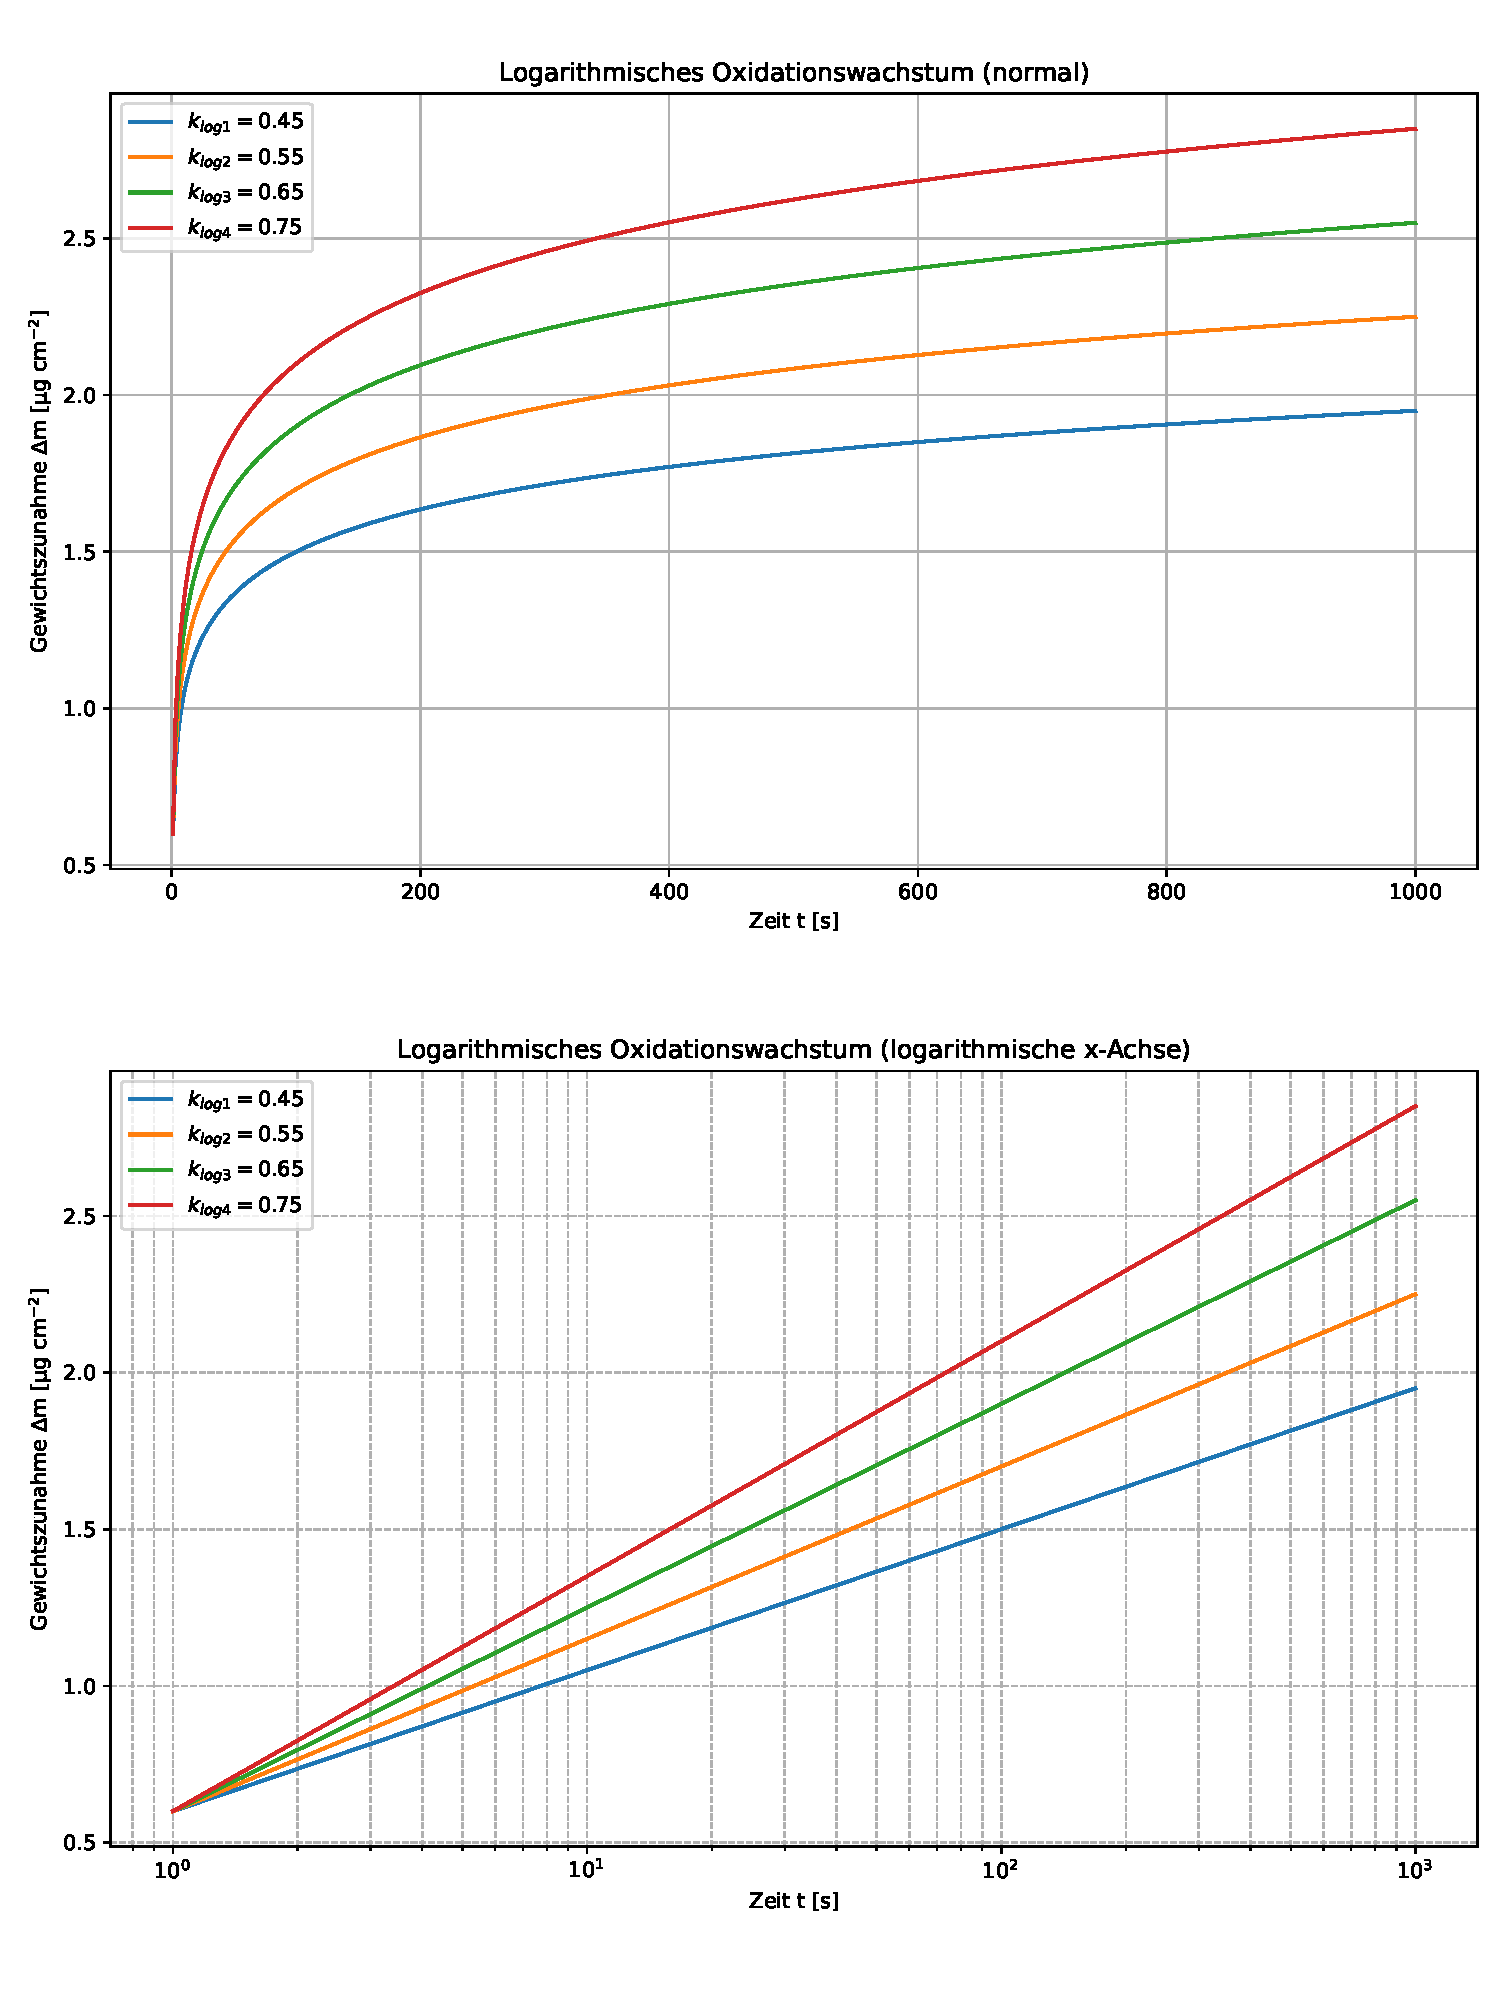
\includegraphics[width=\textwidth, page=1]{img/21/Plots_oxi.pdf}
    \caption{Entstandene Graphen aus der Gleichung, die in der Studie gegeben ist, mit verschiedenen $k_log$ konstanten und "Start"oxidation von 0,6.}
    \label{fig:log_3}
\end{figure}
\twocolumn

\listoffigures
\cleardoublepage

\listoftables
\cleardoublepage

% Beispielhafte Zitierung, damit keine Fehlermeldeung entsteht lol
\cite{demtroeder17}

\bibliographystyle{alpha}
\bibliography{Literaturverzeichnis}

\end{document}